\section{Human to Human Handover}
\label{sec:human}

In this section we describe the human-human experiments performed, the different objects, and the acquired data for analysis of handover motions. The section includes analysis of the handover motion in terms of velocity over the trajectory as well as velocity along time, followed by an overall discussion on the different types of handover motions. 

\subsection{Experimental Scenario}

The HHI dataset was gathered as a collaboration between 
École polytechnique fédérale de Lausanne (EPFL) and Karlsruher Institut für Technologie (KIT) \cite{starke_force_2019}. It involves two humans interacting with an object whether to grasp and handover to one another, or to manipulate and place it on a table. The focus of this work is solely on the handover motion. Figure \ref{fig:epfl_dataset} shows a frame of the handover trajectory of the different cups for each of the participants. The experiments includes data of 4 participants, all male, age between 25-35 years old, with a graduate academic background. The recorded data includes motion tracking markers from the OptiTrack system on the participant's wrist and on the cups, as well as data gloves from the CyberGlove system on the participant's hand (not used in this work).

    \begin{figure}
        \centering
        \begin{tabular}{@{}c@{}}
            \centering
            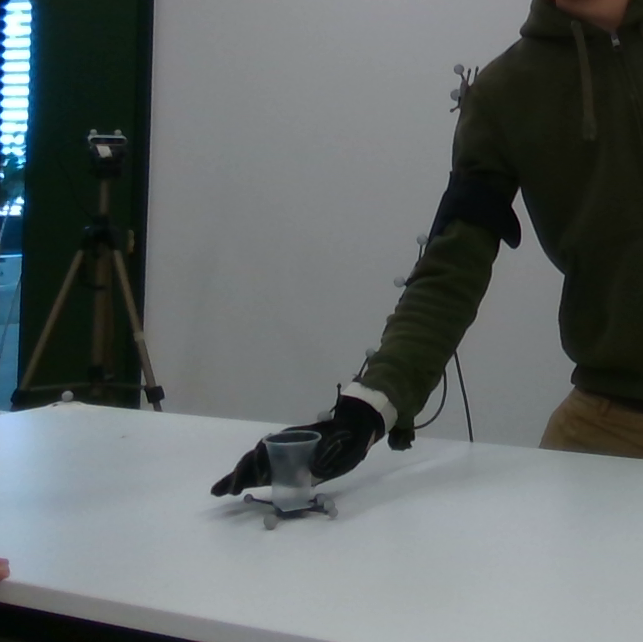
\includegraphics[width=0.225\textwidth,height=0.15\textheight]{Images/frame000023.png}
        \end{tabular}
        \begin{tabular}{@{}c@{}}
            \centering 
            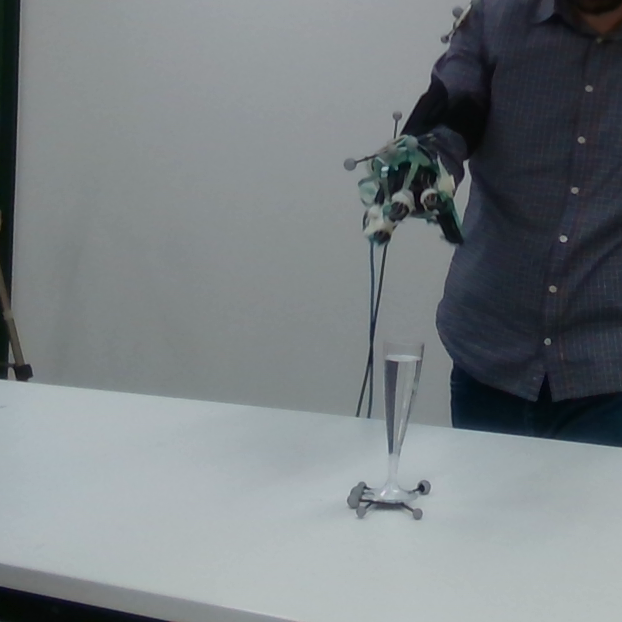
\includegraphics[width=0.225\textwidth,height=0.15\textheight]{Images/frame000046.png}
        \end{tabular}
        \baselineskip
        \begin{tabular}{@{}c@{}}
            \centering 
            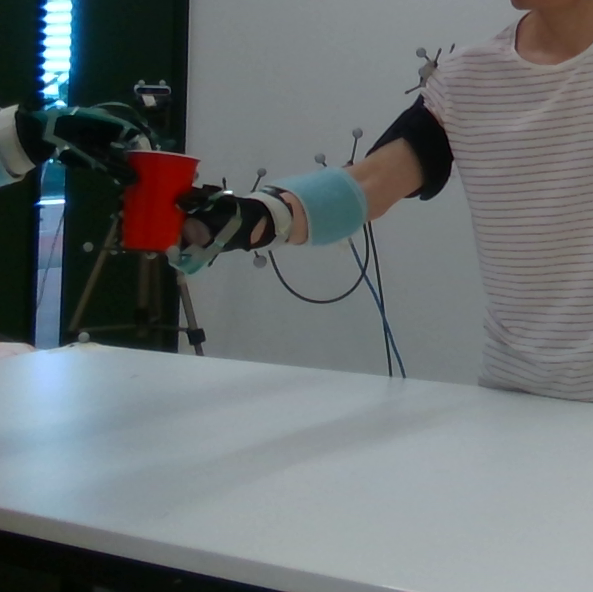
\includegraphics[width=0.225\textwidth,height=0.15\textheight]{Images/frame000117.png}
        \end{tabular}
        \begin{tabular}{@{}c@{}}
            \centering 
            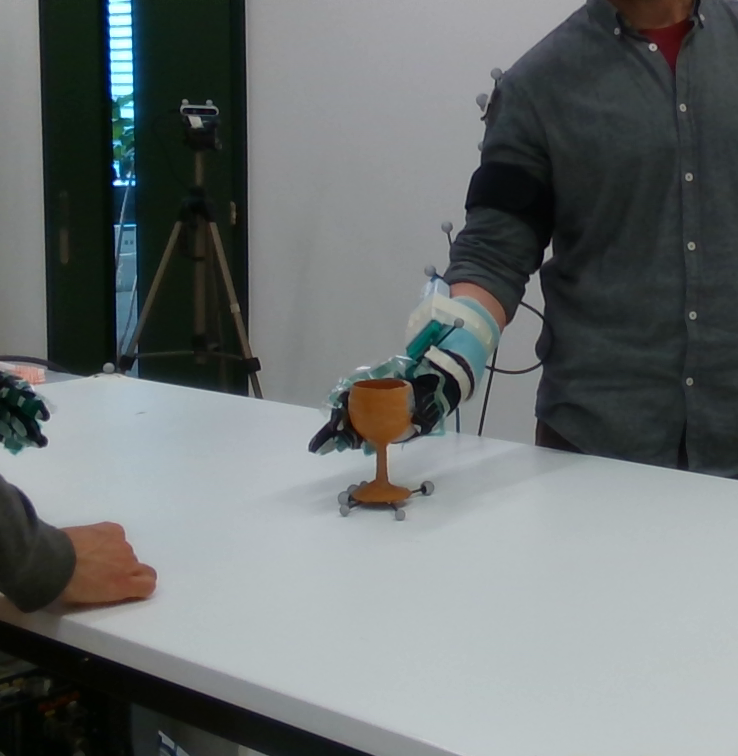
\includegraphics[width=0.225\textwidth,height=0.15\textheight]{Images/frame000144.png}
        \end{tabular}
        \caption{The 4 participants with the 4 cups}
        \label{fig:epfl_dataset}
    \end{figure}
    
The handovers of the cups happen under two distinct situations: (i) an empty cup, and (ii) a cup 90\% filled with water. Each participant hands-over the different cups to a second participant (also present in the dataset but not analysed during the handover), and each cup is manipulated for both conditions. The cups relevant for this work are the red plastic cup (bottom-left), the transparent plastic cup (top-left), the champagne plastic cup (top-right), and the opaque wine glass (bottom-right). The handover trajectory is recorded at 120 Hz, taking on average 1-3 seconds, corresponding to 100-300 data points. A total of 100 handover trajectories are segmented for all the participants with the 4 cups in the two conditions.

The purpose of performing these experiments has to do with the lack of available datasets on human manipulating cups with different internal properties, such as material composition, shape, weight, and with varying conditions such as liquid level. There is also not been, to our knowledge, an extensive analysis on the impact of those varying properties on the kinematic control approaches of humans and possible applications to robots. 

\subsection{Handover Motion Analysis}

The handover motions are 3D Cartesian coordinates over time which begin at the moment of pickup (grasp) and finish when the cup is safely held by the other participant (handover). During the HHI experiments the participant could grasp the cup irrespective of the hand configuration and the handover location could be in whatever 3D space bounded by the table separating the two interactants. This gave rise to several different grasp configurations and a disparity on the duration/length of the handover trajectories. Bear in mind that it was not possible to re-grasp the cup or change grasp configuration during the handover, and the cup would have to start upwards on the table for every interaction. 

    \begin{figure}
        \centering
        \begin{tabular}{@{}c@{}}
            \centering
            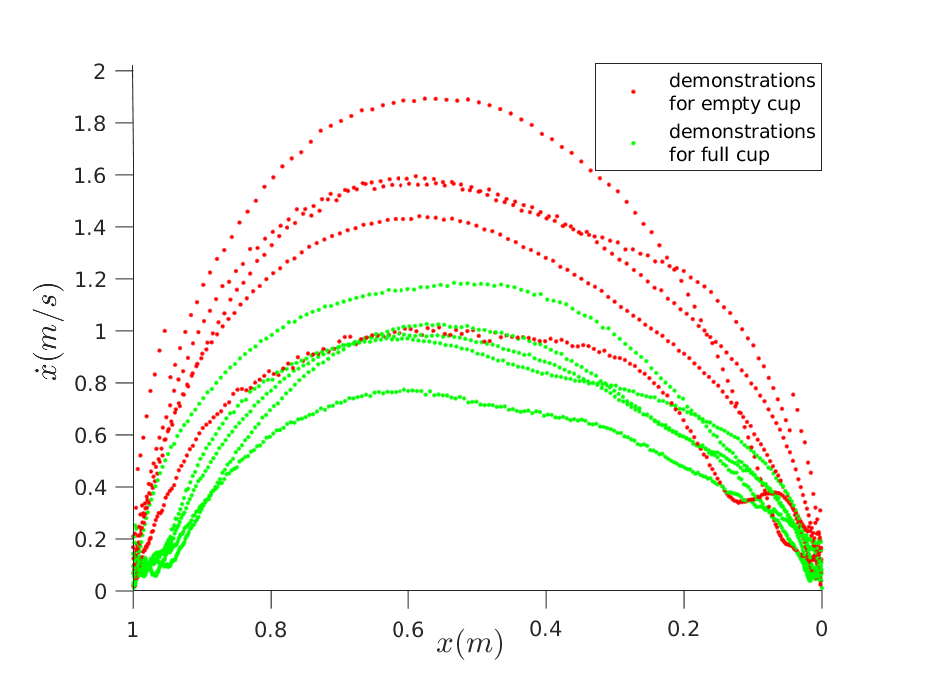
\includegraphics[width=0.48\textwidth,height=0.25\textheight]{Images/vel_distance_plot.eps}
        \end{tabular}
        \baselineskip
        \begin{tabular}{@{}c@{}}
            \centering 
            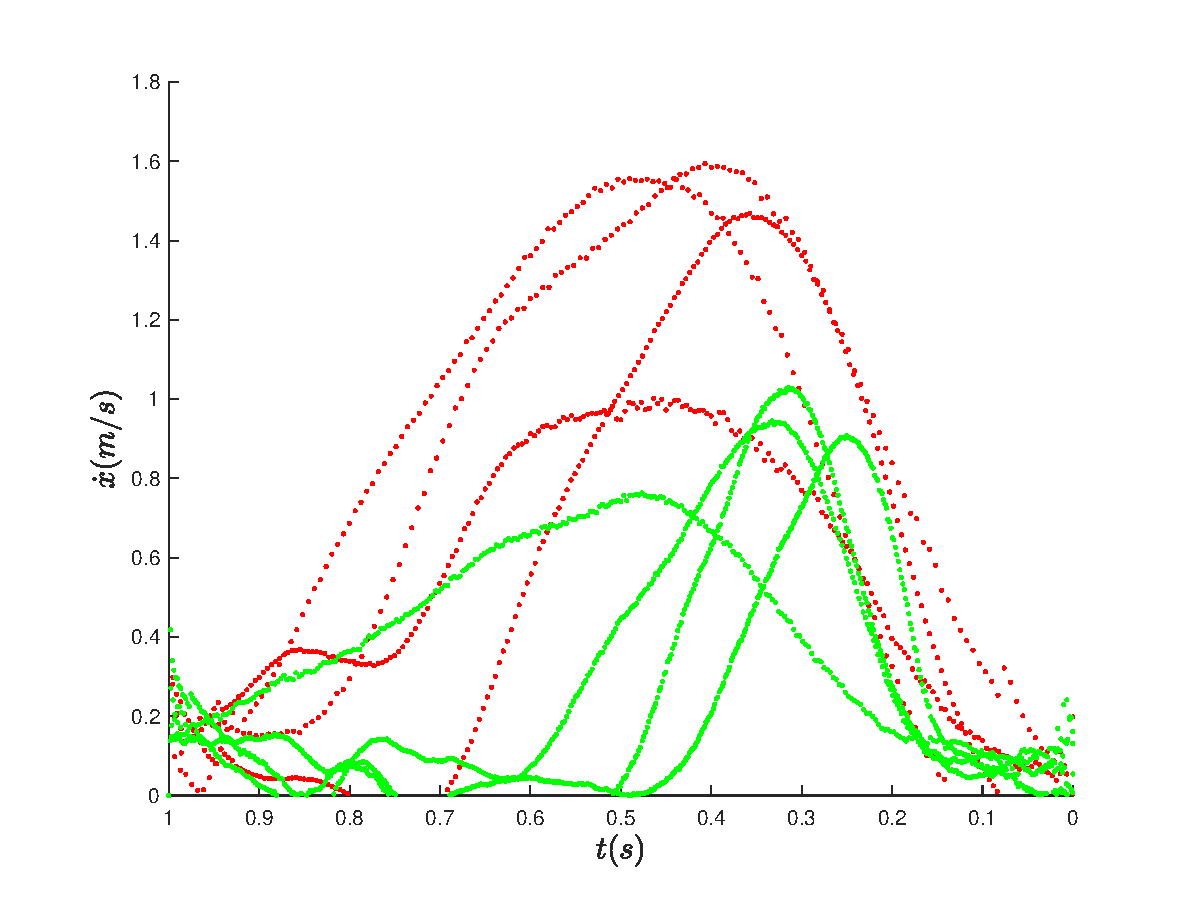
\includegraphics[width=0.48\textwidth,height=0.25\textheight]{Images/vel_time_plot.eps}
        \end{tabular}
        \caption{Sample of the dataset. Velocity/distance (top) and velocity/time (bottom).}
        \label{fig:vel_distance_time}
    \end{figure}

To capture the kinematic of the wrist for all the trials of every participant, cup, and cup condition, irrespective of the starting location in the grasp and the final position for the handover, it was decided to apply min-max normalization before reducing the dimensionality to 1-D vector by calculating the euclidean norm of the $x, y,$ and $z$ dimensions. This re-scales the data to the range [0, 1] where 0 is the final step, refer to as the handover, and 1 is the initial step, refer to as the grasp of the cup from the table. Figure \ref{fig:vel_distance_time} depicts handover trajectories, after post-processing, with respect to the first derivative of the euclidean norm. The plot on the top exhibits the kinematic evolution of the human wrist with respect to the position in the handover trajectory. The bottom plots exhibits the same dataset sample of demonstrations and it represents the velocity of the human wrist with respect to time during the handover trajectory. The purpose of these representations is to identify the acceleration and deceleration phase which is of relevance to the approaches presented in the next section. 

\subsection{Discussion}

The common trait of all demonstrations is the typical bell-shape for the velocity profile as humans choose a minimum jerk approach for the hand trajectory. This has been identified in previous works in point-to-point human motion \cite{flash} and this behaviour manifests, likewise, in human object handovers. In contrast, the most notable difference is on the bell-shape's peak, i.e. the maximum velocity reached by the human. As seen in the demonstrations, the difference can be noticed when distinguishing the cups by the level of water contents, as most of the handovers of empty cups reached higher maximum velocities as the handovers of the same cup full of water. The reason is straightforward as a cup filled with water presents an additional challenge during manipulation: transporting the contents inside without spilling or breaking. There is also the added weight of the liquid to the overall mass of the cup, however we argue that the effect of a liquid moving inside a cup due to the oscillations of the human manipulation is more impactfull in deterring quick and jerky movements than a particular heavy object. Additionally, humans tend to build preconceptions of their surroundings and before manipulation tend to estimate the object's mass and the required force to lift and manipulate. As a result, a novel object with an unexpected heavy mass might invoke a slower manipulation in the first encounter but after some attempts, the human adapts the motor control approach and the manipulation can be more natural. This familiarity procedure is not present when manipulating cups with liquid inside, as the content is visible from the first encounter but the risk of spilling is constantly present. For this reason, we consider the level of water to be the most important factor. In Section \ref{sec:results} we will discuss in depth the different cups and the impact of water contents. 

In this section we 
- we post-process the data
- we notice a difference
- a model the data to note those differences
- resume what you see from the data analysis of the human wrist

